While the simple Texter produces good evaluation results and does return a prioritized list of predicted facts, its predictions miss the desired explanation of why a fact is suggested. At this point, the attentive Texter extends the simple model by an attention mechanism that compares an entity's sentences to each other, forcing the model to favor sentences that are most relevant to the prediction of a certain fact. It is hoped that the added attention mechanism adds the ability to provide an explanations for its predictions, while also increasing the Texter's performance on datasets with multiple sentences per entity.

Technically, the attention mechanism is implemented as an attention block between the embedding and the classification blocks as shown in Figure~\ref{fig:4_approach/1_texter/3_attention_model/attention_architecture}. The embedding block is the same one used in the simple model, leveraging the DistilBERT encoder's contextual word embeddings to support marked input sentences and produce meaningful sentence embeddings. The classification differs slightly from the simple Texter to suit the characteristics of its new input.

\begin{figure}[t]
    \makebox[\textwidth][c]{
        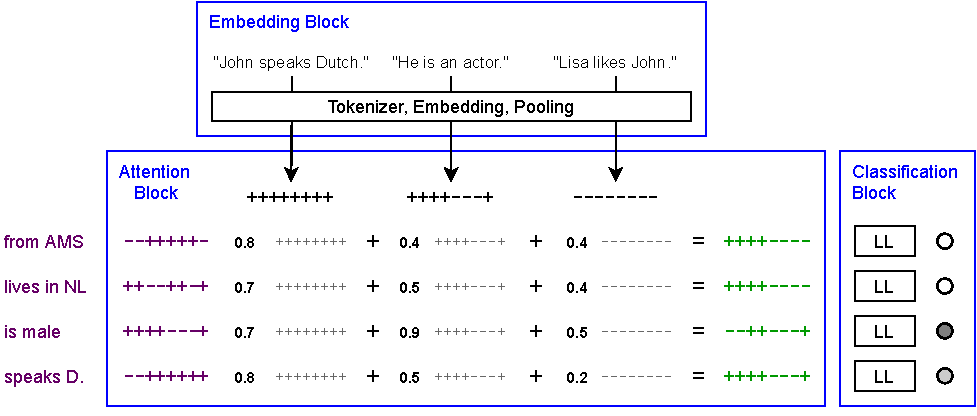
\includegraphics{4_approach/1_texter/3_attention_model/attention_architecture}
    }
    \caption{Attentive Texter architecture: Compared to the simple version, an additional attention block determines the attention of each class embedding (purple) towards each sentence embeddings (black) to weight the sentence embeddings properly when summing them up to class-wise entity embeddings (green) that are then passed to the slightly modified classification block. Classes are abbreviated, e.g. $(x, born~in, Amsterdam)$ to "from AMS".}
    \label{fig:4_approach/1_texter/3_attention_model/attention_architecture}
\end{figure}

Starting by embedding an entity's sentences the same way the simple Texter does, the attentive version then deviates by passing the sentence embeddings to the attention block which contains so-called \emph{class embeddings} -- learnable embeddings of the same dimension as the sentence embeddings that represent the model's classes. When the model is trained, they converge towards word embeddings that are typical for the respective class. During inference, they are compared to the input senence embeddings whereby they best match sentences that contain class-related keywords. Formally, given the set of input sentences $S$ and the set of classes $C$, the similarity between a $d$-dimensional class embedding $\textbf{class}_c \in \mathbb{R}^d$ and a $d$-dimensional sentence embedding $\textbf{sent}_s \in \mathbb{R}^d$ with $1 <= c <= |C|$ and $1 <= s <= |S|$ is calculated as the scalar product $\langle \textbf{class}_c, \textbf{sent}_s \rangle$ between the class and the sentece embedding. Given all class-sentence similarities for a certain class, the model can focus on -- or attend to -- the best matching sentence for that class. Therefore, those similarity values are also referred to as attention values. The attention values are furthermore normalized using the sigmoid function. Thus, the total $|C| \times |S|$ attention matrix $A$ containing the attention values for all combinations of classes from $C$ and sentences from $S$ is calculated as:

\begin{align}
    A_{cs} = \sigma(\langle \textbf{class}_c , \textbf{sent}_s \rangle) && 1 <= c <= |C|,~1 <= s <= |S|
    \label{eq:4_approach/1_texter/3_attention_model/attention_matrix}
\end{align}

In the next step, the attention values are used to combine the sentence embeddings to class-wise entity embeddings $\textbf{ent}_c \in \mathbb{R}^d$. As illstrated in Figure~\ref{fig:4_approach/1_texter/3_attention_model/attention_architecture} and formalized in Equation~\ref{eq:4_approach/1_texter/3_attention_model/ent_emb}, each sentence is weighted by its class-specific attention value. The weighted sentences are then summed up to form class-wise entity embeddings whose purpose is to capture primarily those texts most relevant to the prediction of the respective class. Different from the simple Texter, the entity embeddings are then passed to the subsequent classification block instead of the original sentence embeddings.

\begin{align}
    ent_c = \sum_{s = 1}^{|S|} A_{cs} \cdot sent_s && 1 <= c <= |C|,~1 <= s <= |S|
    \label{eq:4_approach/1_texter/3_attention_model/ent_emb}
\end{align}

Similar to the simple Texter, the attentive Texter's classification layer consists of a $|C| \times d$ weight matrix $W$ and a bias vector $b \in \mathbb{R}^d$. In contrast to the simple model, however, given an entity embedding for a certain class, the weight matrix is not trained with respect to all output classes at once, but only with respect to the regarded class' ground truth output as illustrated in Figure~\ref{fig:4_approach/1_texter/3_attention_model/multi_linear}.  Conceptually, this can be seen as training a separate single-output linear layer for each class and combining the outputs to the multi-label output thereafter as indicated in Figure~\ref{fig:4_approach/1_texter/3_attention_model/attention_architecture}. Formally, the model's output classification logits can be calculated as $\textbf{out}_c = \langle ent_c, W_c \rangle + \textbf{b}_c$ where $W_c$ and $\textbf{b}_c$ are the class' row in the weight matrix and its bias, respectively. The described approach to training the weight matrix was chosen, because an entity embedding for a certain class focuses on the prediction of only that class and would hinder the learning process for other output classes it cannot make a qualified statement about.

\begin{figure}[t]
    \centering
    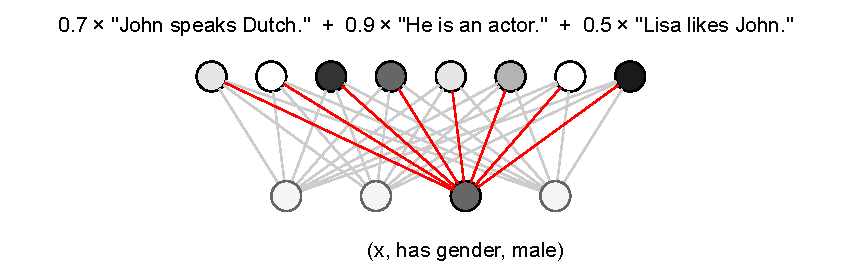
\includegraphics{4_approach/1_texter/3_attention_model/multi_linear}
    \caption{In case of the attentive Texter, the classification block's linear layer is trained w.r.t. a single output class, because the input entity embedding is not helpful for training other classes.}
    \label{fig:4_approach/1_texter/3_attention_model/multi_linear}
\end{figure}

Similar to the simple Texter, the attentive Texter applies the sigmoid activation function to the output logits and takes all classes whose resulting confidences are greater than 50\% to form facts that contain the query entity as their head. In addition to the simple Texter, however, the attentive model provides the facts with the sentence weights as they result from the attention matrix in order to provide the user with an explanation for each fact's prediction. So, in the example, the fact $(John, has~gender, male)$, with a probability around 70\%, would be accompanied by the information that it was primarily suggested due to the sentence "He is an actor.", followed by "John speaks Dutch." and lastly "Lisa likes John.".
